\clearpage
\section{Cautionary Tale on Filtering}
\label{filtering}

It is tempting to insert standard filtering techniques from signal processing 
after creating a Gaussian process model but prior to any dynamic time warping 
calculations. A fast Fourier transform (FFT) based low-pass filter 
\cite{merletti1999standards,moreland2003fft} or 
Mel-frequency cepstral coefficients (MFCC) \cite{muda2010voice,imai1983cepstral} could be used to reduce error 
in the model itself, 
and thus make the contribution FOM more precise. Unfortunately, most 
fuel cycle metrics are not well-formed candidates for such filtering strategies.
Including such filters as part of the analysis can easily lead to wildly unphysical
models.

Consider a simple low-pass filter where a 256 channel real-valued FFT frequency 
transform is taken.  All but lowest 32 channels are discarded prior to the applying 
the inverse transform. High frequency jitter in the original signal is removed, 
allowing for a better signal-to-noise ratio.

\begin{figure}[htb]
\centering
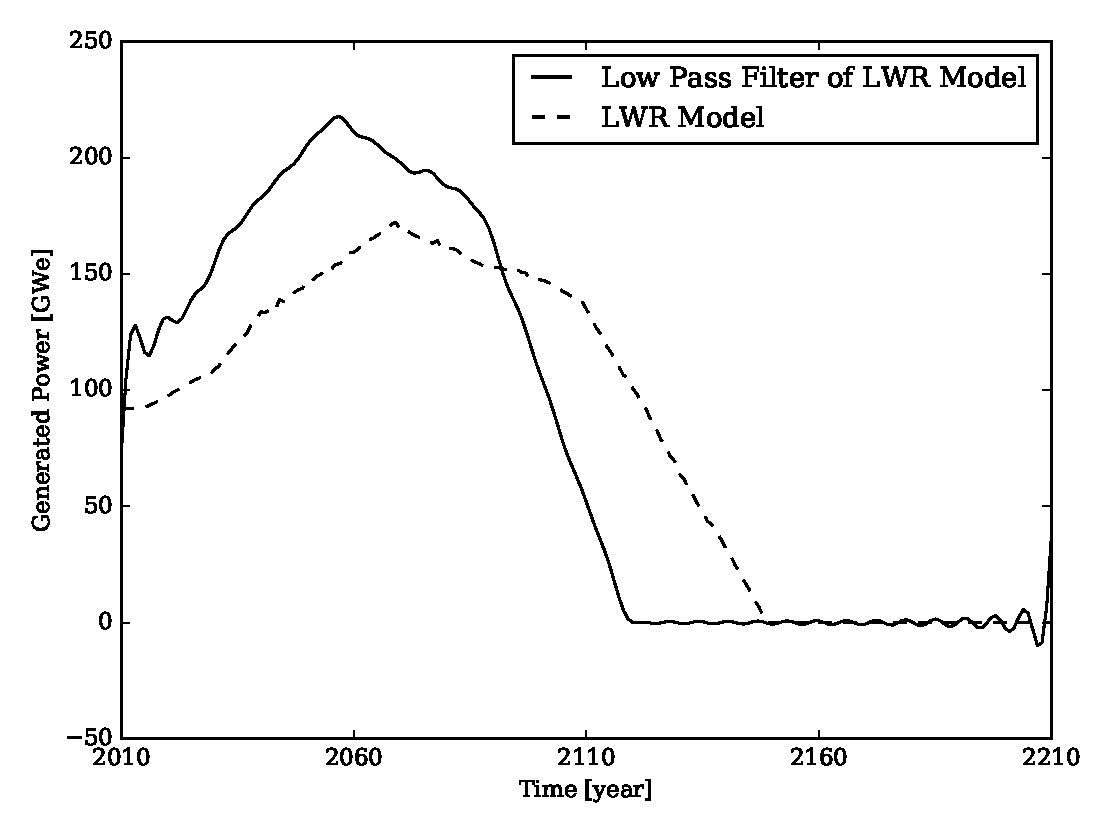
\includegraphics[width=0.9\textwidth]{fft-lwr-model.eps}
\caption{Low-pass FFT filter of LWR Gaussian process model $m_*^\LWR$ alongside
the unfiltered model itself.}
\label{fft-lwr-model}
\end{figure}

Figure \ref{fft-lwr-model} shows the results of applying the low-pass filter 
described above to the Gaussian process model of the generated power from LWRs, 
$m_*^\LWR$.  The filtered curve demonstrates at least three major problems.  The
first is that the values of the curve are allowed to be negative, which is 
impossible for this (and many other) fuel cycle metric.  The second is that 
near the time boundaries ($t=2010$ and $t=2210$), the amplitude of the filtered model
is significantly higher than itself. At $t=2210$, the metric should be zero but
instead is 36.5 GWe. Thirdly, the shape of the curve itself is skewed to lower 
times. The time at which the metric goes to zero should be near year 2150 but is 
instead closer to year 2115.  All of these issues would severely distort any 
DTW calculations that follow.

The reason behind these inconsistencies is that the FFT process is fundamentally 
periodic.  However, using the annual time grid here, most fuel cycle metrics 
are not periodic. Neither is the modeling error for such metrics periodic. 
Thus, while well-intentioned, a low-pass filter is not generally applicable.

Alternatively, MFCCs provide a mechanism for converting a time series into a 
set of power spectrum coefficient curves. Since the dynamic time warping procedure
uses an L1 norm to form the cost matrix, the MFCCs of two signals can be directly 
compared. Each coefficient should roughly correspond in shape and amplitude to some
feature in the original signal.  Noisy, high frequency coefficients tend to be 
very similar and so their contribution to a DTW is less corresponding less than 
lower coefficients. Coupling MFCC to DTW is an extremely common method employed in 
speech recognition systems.  

\begin{figure}[htb]
\centering
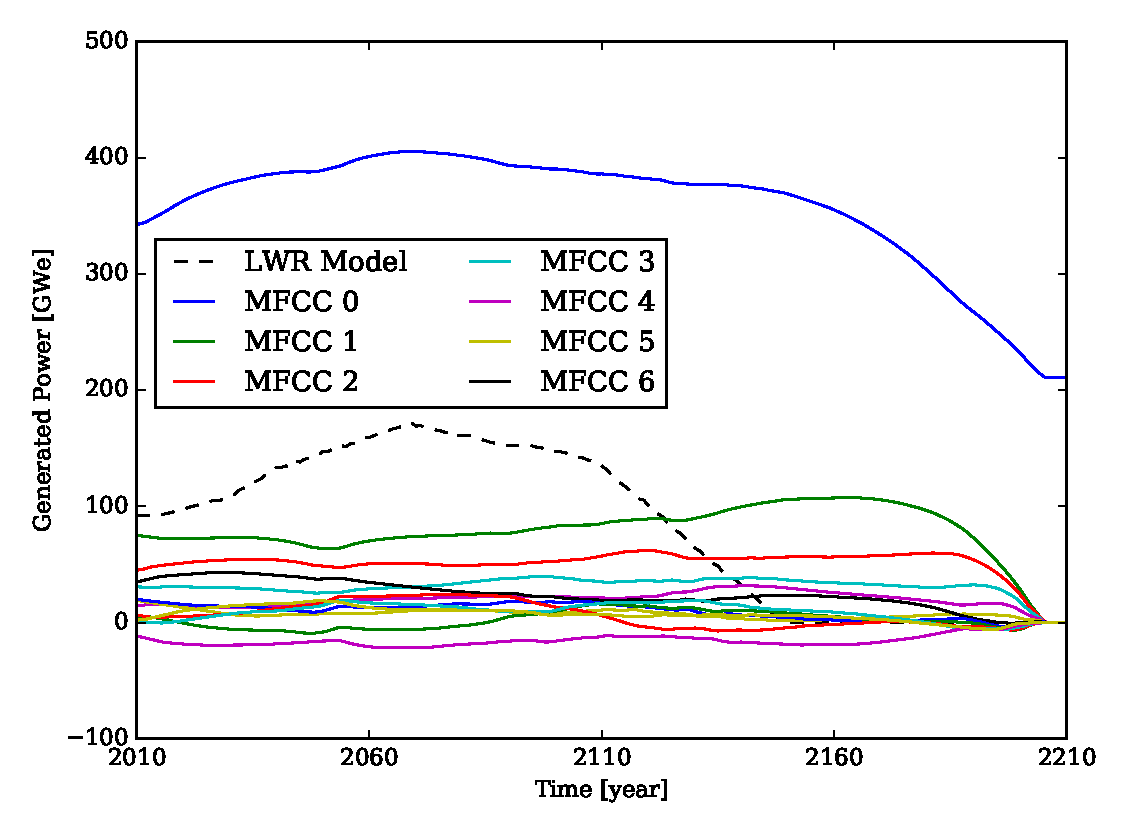
\includegraphics[width=0.9\textwidth]{mfcc-lwr-model.eps}
\caption{Representative Mel-frequency cepstral coefficients (solid lines) of an 
LWR Gaussian process model $m_*^\LWR$ alongside the model itself (dashed line).}
\label{mfcc-lwr-model}
\end{figure}

Figure \ref{mfcc-lwr-model} displays the MFCC curves for the LWR Gaussian 
process model with the model itself. None of these curves, not even the major 
coefficient resembles the actual model.  Rather, the cosine basis for MFCCs
are clearly visible.  As with the low-pass filter, the MFCCs also have 
uncharacteristic negative components.  Moreover, 
the metric data is not sampled frequently enough to have meaningful
time windows. For fuel cycle metrics here, there is one data point per year for 
where the signal itself may change in a meaningful way each year. By comparison, 
in speech recognition, audio is sampled at least at 22050 Hz for characteristic 
signals on the order of 1 second.  The data volume for fuel cycle benchmark metrics
is simply too low for MFCC transformations to be applicable. 

Still, suppose the contribution measure is computed for the MFCCs of LWR, FR, and 
total generated power models.  In this case the LWR contribution is found to be 
0.572 while the FR contribution is 0.899. Using the models directly as was done 
in \S\ref{contribution}, the contribution values were 0.298 and 0.859 respectively.
This implies that using the MFCCs had the opposite effect as desired.  The MFCCs
added error to the system and mad the LWR and FR contributions seem more alike than 
they truly are.

Therefore filtering the models prior to dynamic time warping is a dubious practice
in the general case. In all likelihood, the metric does not meet the underlying 
assumptions of the filter. The metric may not be periodic or may not be sampled 
frequently enough. Sometimes it may be possible to construct as metric that does
meet these qualifications, such as if the generated power is sampled monthly and 
seasonal demand behavior is noticeable. In such a case, it is instead recommended
to pick a different kernel for the Gaussian process model, such that these 
periodic behaviors are captured.  The regression itself then takes on the role of 
minimizing model uncertainty. Further filtering to this end becomes redundant and
dangerous.  Additionally, it is unlikely that 
the majority of the simulators would be able to calculate such a high-fidelity metric.
That alone should disqualify such a metric from any benchmarking study or
inter-code comparison.
